\documentclass[tikz,border=4pt]{standalone}
\usepackage[scaled=.92]{helvet}
\usepackage{sansmath,amssymb}
\usepackage[no-math]{fontspec}
\IfFontExistsTF{Arial}{\setsansfont{Arial}}{\setsansfont{Liberation Sans}}
\usetikzlibrary{arrows.meta,positioning,shapes.geometric}
\begin{document}
\sffamily\sansmath
\begin{tikzpicture}[
    node distance=0.3cm and 0.5cm,
    inputbox/.style={trapezium, trapezium left angle=70, trapezium right angle=110,
                     draw, very thick, fill=cyan!8, minimum width=1.3cm,
                     minimum height=0.8cm, align=center, text depth=0pt, font=\normalsize\bfseries\linespread{.85}\selectfont},
    outputbox/.style={trapezium, trapezium left angle=110, trapezium right angle=70,
                      draw, very thick, fill=red!30, minimum width=1.1cm,
                      minimum height=0.8cm, align=center, text depth=0pt, font=\normalsize\bfseries},
    mainbox/.style={rectangle, draw, very thick, rounded corners=4pt,
                    minimum width=1.4cm, minimum height=0.9cm,
                    align=center, text depth=0pt, font=\normalsize\bfseries\linespread{.85}\selectfont},
    detailbox/.style={rectangle, draw, thick, rounded corners=3pt,
                      minimum width=1.1cm, minimum height=0.7cm,
                      align=center, text depth=0pt, font=\footnotesize\linespread{.85}\selectfont},
    smalldetail/.style={rectangle, draw, thick, rounded corners=3pt,
                        minimum width=0.9cm, minimum height=0.6cm,
                        align=center, text depth=0pt, font=\footnotesize\linespread{.85}\selectfont},
    smalldetailbold/.style={rectangle, draw, thick, rounded corners=3pt,
                            minimum width=0.9cm, minimum height=0.6cm,
                            align=center, text depth=0pt, font=\footnotesize\bfseries\linespread{.85}\selectfont},
    gatecircle/.style={circle, draw, very thick, minimum size=0.8cm,
                       font=\LARGE\bfseries},
    smallcirc/.style={circle, draw, thick, minimum size=0.6cm, font=\normalsize},
    arrow/.style={->, >={Stealth[length=2mm, width=1.5mm]}, very thick},
    thinarrow/.style={->, >={Stealth[length=1.5mm, width=1.5mm]}, thick},
    dashedarrow/.style={->, >={Stealth[length=2.5mm, width=1.5mm]}, thick, dashed, black},
    dashdotarrow/.style={->, >={Stealth[length=1.5mm, width=1.5mm]}, thick, black,
                         dash pattern=on 1pt off 3pt on 0.8pt off 2pt},
]


\node[inputbox] (input) at (0,0) {Input\\$\mathbf{x}_i$};
\node[mainbox, fill=blue!10, right=0.5cm of input] (moiety_enc) {MOTIF};
\node[mainbox, fill=purple!10, right=0.5cm of moiety_enc] (molecule) {Molecule\\Layer};
\node[gatecircle, fill=green!12, right=0.5cm of molecule] (gate1) {$\odot$};
\node[mainbox, fill=orange!12, right=0.5cm of gate1] (form_attn)
     {Formulation\\Attention};
\node[mainbox, fill=purple!10, right=0.5cm of form_attn] (pool) {Pool};
\node[gatecircle, fill=green!15, right=0.5cm of pool] (gate2) {$\odot$};
\node[mainbox, fill=red!10, right=0.5cm of gate2] (mlp) {MLP};
\node[outputbox, right=0.5cm of mlp] (output) {$\hat{y}$};

\draw[arrow] (input) -- (moiety_enc);
\draw[arrow] (moiety_enc) -- (molecule);
\draw[arrow] (molecule) -- (gate1);
\draw[arrow] (gate1) -- (form_attn);
\draw[arrow] (form_attn) -- (pool);
\draw[arrow] (pool) -- (gate2);
\draw[arrow] (gate2) -- (mlp);
\draw[arrow] (mlp) -- (output);

\node[smalldetail, fill=purple!8, minimum height=0.75cm, above=0.6cm of molecule] (mol_detail)
     {Shared MLP\\Sum pooling};
\node[smalldetailbold, fill=green!10, minimum height=0.75cm, above=0.6cm of gate1] (mr_enc)
     {Molar Ratio\\Encoder};
\node[smalldetail, fill=orange!10, minimum height=0.75cm, above=0.6cm of form_attn] (mha) {MHA};
\node[smalldetail, fill=purple!8, minimum height=0.75cm, above=0.6cm of pool] (pool_detail) {Masked\\Avg};
\node[smalldetailbold, fill=green!12, minimum height=0.75cm, above=0.6cm of gate2] (temp_enc)
     {Temperature\\Encoder};

\draw[dashedarrow] (mol_detail.south) -- (molecule.north);
\draw[dashedarrow] (mha.south) -- (form_attn.north);
\draw[dashedarrow] (pool_detail.south) -- (pool.north);

\draw[thinarrow, green!60!black] (mr_enc.south) -- (gate1.north);
\draw[thinarrow, green!60!black] (temp_enc.south) -- (gate2.north);

\draw[dashdotarrow, black] (input.north) -- ++(0,2.0) -|
                          ([yshift=0.2cm]mr_enc.north) -- (mr_enc.north);
\draw[dashdotarrow, black] (input.north) -- ++(0,2.0) -|
                          ([yshift=0.2cm]temp_enc.north) -- (temp_enc.north);

\node[below=0.03cm of gate1, xshift=0.1cm, font=\small, text=teal!90] {$\mathbf{G}_{mr}$};
\node[below=0.03cm of gate2, xshift=0.1cm, font=\small, text=teal!90] {$\mathbf{g}_{temp}$};

\begin{scope}[xshift=-4.0cm, yshift=-5.0cm]

\node[detailbox, fill=blue!8] (h_in) at (5.88,1.5) {$\mathbf{H}^{(l)}$};

\node[font=\small\bfseries, text=blue!70, align=left, anchor=west] (dual_title)
     at (15.8,3)
     {Dual Attention Mechanism\\
      within each MOTIF layer\\
      $l \in [1,L]$};

\node[smallcirc, fill=gray!20, right=0.6cm of h_in] (split) {$\divideontimes$};

\node[detailbox, fill=gray!20, above right=0.5cm and 0.4cm of split] (h_l)
     {$\mathbf{H}_l$};
\node[above=0.01cm of h_l, font=\footnotesize, text=black] {LOCAL};

\node[smalldetail, fill=red!20, right=0.8cm of h_l] (local_q) {$\mathbf{Q}_l$};
\node[smalldetail, fill=red!20, above=0.02cm of local_q] (local_k) {$\mathbf{K}_l$};
\node[smalldetail, fill=red!20, below=0.02cm of local_q] (local_v) {$\mathbf{V}_l$};

\node[detailbox, fill=orange!25, right=0.5cm of local_q, rounded corners=5pt]
     (local_matmul) {Matmul\\$+\mathbf{A'}$};
\node[below=0.03cm of local_matmul, xshift=0.4cm, inner sep=0.5pt] (adj_mat) {
    \begin{tikzpicture}[scale=0.2]
        \fill[red!60] (0,0) rectangle (1,1);
        \fill[red!60] (1,0) rectangle (2,1);
        \fill[white!40] (2,0) rectangle (3,1);
        \fill[red!60] (0,1) rectangle (1,2);
        \fill[red!60] (1,1) rectangle (2,2);
        \fill[white!40] (2,1) rectangle (3,2);
        \fill[white!40] (0,2) rectangle (1,3);
        \fill[white!40] (1,2) rectangle (2,3);
        \fill[red!60] (2,2) rectangle (3,3);
        \draw[thin, black] (0,0) grid (3,3);
    \end{tikzpicture}
};

\node[detailbox, fill=orange!18, right=0.5cm of local_matmul] (z_l) {$\mathbf{Z}_l$};

\node[detailbox, fill=gray!20, below right=0.5cm and 0.4cm of split] (h_g)
     {$\mathbf{H}_g$};
\node[above=0.01cm of h_g, font=\footnotesize, text=black] {GLOBAL};

\node[smalldetail, fill=cyan!15, right=0.8cm of h_g] (global_q) {$\mathbf{Q}_g$};
\node[smalldetail, fill=cyan!15, above=0.02cm of global_q] (global_k) {$\mathbf{K}_g$};
\node[smalldetail, fill=cyan!15, below=0.02cm of global_q] (global_v) {$\mathbf{V}_g$};

\node[detailbox, fill=teal!30, right=0.5cm of global_q, rounded corners=5pt]
     (global_matmul) {Matmul\\$\odot\mathbf{D}'$};
\node[below=0.02cm of global_matmul, inner sep=0.5pt, xshift=0.4cm] (dist_mat) {
    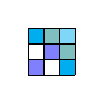
\begin{tikzpicture}[scale=0.2]
        \fill[blue!50] (0,0) rectangle (1,1);
        \fill[white] (1,0) rectangle (2,1);
        \fill[cyan] (2,0) rectangle (3,1);
        \fill[white] (0,1) rectangle (1,2);
        \fill[blue!50] (1,1) rectangle (2,2);
        \fill[teal!50] (2,1) rectangle (3,2);
        \fill[cyan] (0,2) rectangle (1,3);
        \fill[teal!50] (1,2) rectangle (2,3);
        \fill[cyan!50] (2,2) rectangle (3,3);
        \draw[thin, black] (0,0) grid (3,3);
    \end{tikzpicture}
};

\node[detailbox, fill=teal!18, right=0.5cm of global_matmul] (z_g) {$\mathbf{Z}_g$};

\node[smallcirc, fill=gray!8, right=6.2cm of split] (concat) {$\oplus$};
\node[detailbox, fill=blue!10, right=0.5cm of concat] (add_norm) {Add \&\\Norm};
\node[detailbox, fill=blue!10, right=0.5cm of add_norm] (h_out) {$\mathbf{H}^{(l+1)}$};

\draw[thinarrow] (h_in) -- (split);
\draw[thinarrow] (split.north) |- (h_l.west);
\draw[thinarrow] (h_l) -- (local_k);
\draw[thinarrow] (h_l) -- (local_q);
\draw[thinarrow] (h_l) -- (local_v);
\draw[thinarrow] (local_k) -| ([xshift=-0.35cm]local_matmul.north);
\draw[thinarrow] (local_q) -- (local_matmul);
\draw[thinarrow] (local_v) -| ([xshift=-0.35cm]local_matmul.south);
\draw[thinarrow] (local_matmul) -- (z_l);

\draw[thinarrow] (split.south) |- (h_g.west);
\draw[thinarrow] (h_g) -- (global_k);
\draw[thinarrow] (h_g) -- (global_q);
\draw[thinarrow] (h_g) -- (global_v);
\draw[thinarrow] (global_k) -| ([xshift=-0.35cm]global_matmul.north);
\draw[thinarrow] (global_q) -- (global_matmul);
\draw[thinarrow] (global_v) -| ([xshift=-0.35cm]global_matmul.south);
\draw[thinarrow] (global_matmul) -- (z_g);

\draw[thinarrow] (z_l.east) -| (concat.north);
\draw[thinarrow] (z_g.east) -| (concat.south);
\draw[thinarrow] (concat) -- (add_norm);
\draw[thinarrow] (add_norm) -- (h_out);

\draw[dashdotarrow] (h_in.south) -- ++(0,-2.3) -|
                    ([yshift=-0.5cm]add_norm.south) -- (add_norm.south);

\node[below=-0.1cm of adj_mat, font=\footnotesize, text=black] {Adjacency $\mathbf{A}$};
\node[below=-0.1cm of dist_mat, font=\footnotesize, text=black] {Distance $\mathbf{D}$};

\end{scope}

\draw[dashedarrow, blue!70] (moiety_enc.south) -- (h_in.north);

\end{tikzpicture}
\end{document}
